 \documentclass{report}
 
\usepackage[utf8]{inputenc} 
\usepackage[T1]{fontenc}      
\usepackage[top=2.0cm, bottom=3cm, left=3.0cm, right=3.0cm]{geometry}
\usepackage{graphicx}
\usepackage{wrapfig}
\usepackage{amsmath,esint }
\usepackage{amssymb}
\graphicspath{{figures/}{../figures}}

\newcommand*\dif{\mathop{}\!\mathrm{d}}
\newcommand*\diver{\mathop{}\!\mathrm{div}}
\newcommand*\grad{\mathop{}\!\mathrm{grad}}

\begin{document}

\section*{Sillage d'un avion}

On considère le vol d'un avion de chasse se déplaçant dans le sens des $x$ croissants, à une vitesse $v$ sur une droite horizontale $(y=0,z=h)$ alors qu'un observateur est situé au point $O(0,0,0)$. L'avion émet un signal sonore de période $T$. On note $\theta=\vec{Ox},\vec{OA})$ l'inclinaison par rapport à l'horizontale de la direction observateur-avion. Cet angle est supposé varier peu pendant une période $T$.

\begin{itemize}

	\item[$\circ$] L'air a une masse volumique au repos $\rho_0$ et une compressibilité $\chi_s$. Retrouver l'équation d'Alembert caractérisant la propagation des ondes sonores dans l'air, en explicitant la vitesse de propagation $c$ des ondes.

\end{itemize}

On suppose dans un premier temps que l'avion se déplace à une vitesse subsonique, c'est-à-dire $v<c$.

\begin{itemize}

	\item[$\star$] Quelle est la période $T'$ du signal perçu par l'observateur ? Commenter l'expression selon les valeurs prises par $\theta$. Comment s'appelle ce phénomène ?
	
	\item[$\star$] Quelle est la région de l'espace qui peut être atteinte à un instant donné par l'onde sonore provenant de l'avion ?

\end{itemize}

On suppose désormais que l'avion se déplace à une vitesse supersonique, c'est-à-dire $v>c$.

\begin{itemize}

	\item[$\diamond$] Le son émis par l'avion à l'instant $t$ est perçu par l'observateur à l'instant $t'=f(t)$. Déterminer la fonction $f$ si l'avion passe à l'instant $t=0$ à la verticale de l'observateur. Représenter graphiquement $f$.
	
	\item[$\diamond$]  Pourquoi le son perçu est-il particulièrement intense si $\dif t'/\dif t=0$ ? Comment s'appelle ce phénomène ? 
	
	\item[$\diamond$]  On donne $h=1000$m ; $v=500$m.s$^{-1}$ ; $c=340$m.s$^{-1}$. On note $t'_0$ l'instant auquel le bang est perçu par l'observateur et $t_0$ l'instant auquel les sons perçus à l'instant $t'_0$ ont été émis par l'avion. Déterminer $t_0$, $t'_0$ et les positions de l'avion à $t_0$ et $t'_0$. 
	
	\item[$\diamond$] L'observateur entend-il l'avion avant d'entendre le bang ? Quelle est la durée $\Delta t$ d'émission des sons perçus entre $t'_0$ et $t'_0+\Delta t'$ (on pourra effectuer une développement limité de $f(t)$). Calculer $\Delta t$ pour $\Delta t'=0.1$s et commenter.
	
	\item[$\diamond$] Quelle est la région de l'espace qui peut être atteinte à un instant donné par une onde sonore provenant de l'avion ?
	
	\item[$\diamond$] Estimer la vitesse de l'obus en photo ci-dessous.  

\end{itemize}

\begin{figure}[h!]
\centering
		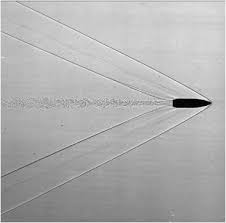
\includegraphics[scale=0.7]{obus.jpg}
\end{figure}

\end{document}
